\documentclass[12pt]{article}
\usepackage[margin=2.5cm]{geometry}
\usepackage{enumerate}
\usepackage{amsfonts}
\usepackage{amsmath}
\usepackage{fancyhdr}
\usepackage{amsmath}
\usepackage{amssymb}
\usepackage{amsthm}
\usepackage{mdframed}
\usepackage{graphicx}
\usepackage{subcaption}
\usepackage{adjustbox}
\usepackage{listings}
\usepackage{xcolor}
\usepackage{booktabs}
\usepackage[utf]{kotex}
\usepackage{hyperref}

\definecolor{codegreen}{rgb}{0,0.6,0}
\definecolor{codegray}{rgb}{0.5,0.5,0.5}
\definecolor{codepurple}{rgb}{0.58,0,0.82}
\definecolor{backcolour}{rgb}{0.95,0.95,0.92}

\lstdefinestyle{mystyle}{
    backgroundcolor=\color{backcolour},
    commentstyle=\color{codegreen},
    keywordstyle=\color{magenta},
    numberstyle=\tiny\color{codegray},
    stringstyle=\color{codepurple},
    basicstyle=\ttfamily\footnotesize,
    breakatwhitespace=false,
    breaklines=true,
    captionpos=b,
    keepspaces=true,
    numbers=left,
    numbersep=5pt,
    showspaces=false,
    showstringspaces=false,
    showtabs=false,
    tabsize=1
}

\lstset{style=mystyle}

\pagestyle{fancy}
\renewcommand{\headrulewidth}{0.4pt}
\lhead{Team Treehouse}
\rhead{Querying Relational Databases Part 2 Notes}

\begin{document}
\title{Querying Relational Databases Part 2 Notes}
\author{Team Treehouse}
\maketitle

\bigskip

\section{Unique Keys}

\bigskip

\begin{itemize}
    \item Is configured so that no value can be repeated
    \item Can be null (if schema permits)
    \item Can have multiple unique keys per table
    \begin{itemize}
        \item e.g. unique emails column, and uniqe ssn column in one table
    \end{itemize}
    \item Can be modified to a new value
    \begin{itemize}
        \item As long as it is not conflicted with others
    \end{itemize}
\end{itemize}

\bigskip

\section{PRIMARY Keys}

\bigskip

\begin{itemize}
    \item Never be null
    \item One primary key per table
    \item Cannot be modified to a new value

    \begin{center}
    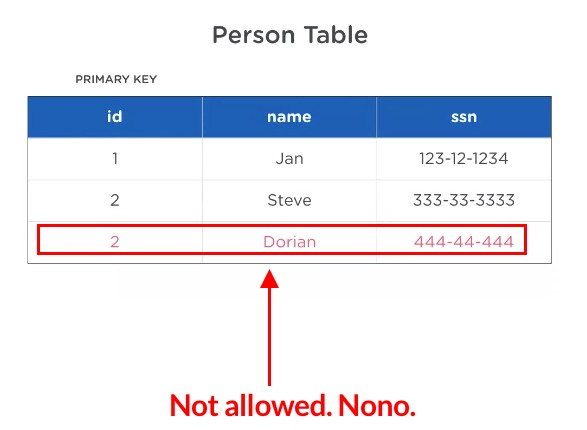
\includegraphics[width=0.7\linewidth]{images/part_2_notes_1.png}
    \end{center}
\end{itemize}

\bigskip

\section{Quiz 1}

\bigskip

\begin{enumerate}[1.]
    \item

    What happens when a Unique Constraint is violated in a database system?

    \bigskip

    \begin{enumerate}[A.]
        \item An email alert is sent to the Database Administrator.
        \item The database locks up until the Database Administrator does a reboot.
        \item The database does not allow the data to be written to the table and an error is returned.
        \item The database allows the data to be written anyway.
    \end{enumerate}

    \bigskip

    \textbf{Answer:} C

    \item

    What data type does a primary key have to be?

    \bigskip

    \begin{enumerate}[A.]
        \item Integer
        \item Text
        \item Either, as long as the value guarantees uniqueness
    \end{enumerate}

    \bigskip

    \textbf{Answer:} C

    \item

    Which of the following is NOT something a database key can do?

    \bigskip

    \begin{enumerate}[A.]
        \item Ensure a value does not repeat within a given column.
        \item Guarantee a table does not return data when queried unless a specific password is supplied.
        \item Guarantee an entire row is unique within a table.
        \item Act as a pointer or a link back to another table.
    \end{enumerate}

    \bigskip

    \textbf{Answer:} B

    \item

    A Primary Key will allow one NULL value, but no more than that.

    \bigskip

    \begin{enumerate}[A.]
        \item True
        \item False
    \end{enumerate}

    \bigskip

    \textbf{Answer:} B

\end{enumerate}

\bigskip

\section{Foreign Keys}

\bigskip

\begin{itemize}
    \item value cannot be added to table with foreign key unless the value exists
    in the table with primary key
    \begin{itemize}
        \item is called \textbf{referential integrity}
    \end{itemize}

    \bigskip

    \begin{center}
    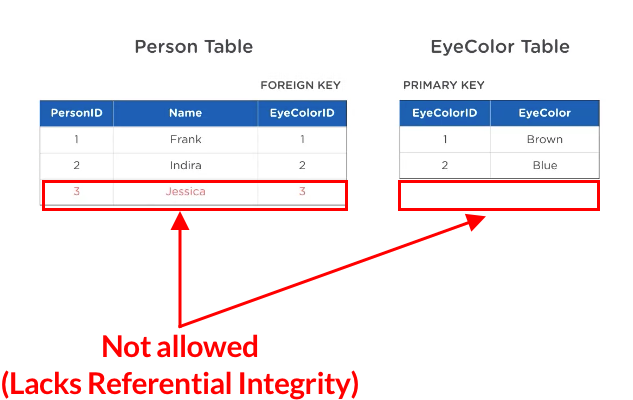
\includegraphics[width=0.8\linewidth]{images/part_2_notes_2.png}
    \end{center}
\end{itemize}

\bigskip

\section{Quiz 2}

\bigskip

\begin{enumerate}[1.]
    \item

    \bigskip

    Assuming 1, 2 and 3 are all values in the primary key table, this is a valid
    Foreign Key column.

    \begin{center}
    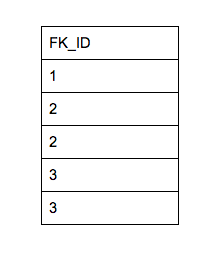
\includegraphics[width=0.4\linewidth]{images/part_2_notes_3.png}
    \end{center}

    \bigskip

    \begin{enumerate}[A.]
        \item True
        \item False
    \end{enumerate}

    \bigskip

    \textbf{Answer:} A

    \item

    \bigskip

    The thing that defines the physical relationship between two tables in a
    database is called:

    \bigskip

    \begin{enumerate}[A.]
        \item Foreign Key View
        \item Foreign Key Constraint
        \item Foreign Key Hole
        \item Foreign Key Page
    \end{enumerate}

    \bigskip

    \textbf{Answer:} B

    \item

    \bigskip

    What are Foreign Keys?

    \bigskip

    \begin{enumerate}[A.]
        \item They are columns that guarantee uniqueness within the table.
        \item They are columns that contain data which relate to the Primary Key in another table.
        \item They are columns that contain international demographic information.
        \item They are keys on a piano that come from another country.

    \end{enumerate}

    \bigskip

    \textbf{Answer:} B

    \item

    If NO Foreign Key Constraint exists between two tables, it is possible to
    accidentally record data in a foreign key column that does not have a matching
    value in the primary key table.

    \bigskip

    \begin{enumerate}[A.]
        \item True
        \item False
    \end{enumerate}

    \bigskip

    \textbf{Answer:} A

    \item

    Once a Foreign Key Constraint is created to enforce the referential
    integrity between two tables, what happens if you try to insert a value that
    does NOT exist in the primary key table?

    \bigskip

    \begin{enumerate}[A.]
        \item It will insert the data anyway.
        \item It will alert the Database Administrator that someone is trying to violate referential integrity and lock the database.
        \item It will NOT insert the data, and will return an error.
    \end{enumerate}

    \bigskip

    \textbf{Answer:} C


\end{enumerate}



\end{document}